\documentclass[tikz,border=5pt]{standalone}
\usepackage{pgfplots}
\pgfplotsset{compat=1.18}

\definecolor{corba}{HTML}{365FB3}
\definecolor{punt}{HTML}{B91C1C}
\definecolor{guia}{HTML}{6B7280}

\begin{document}
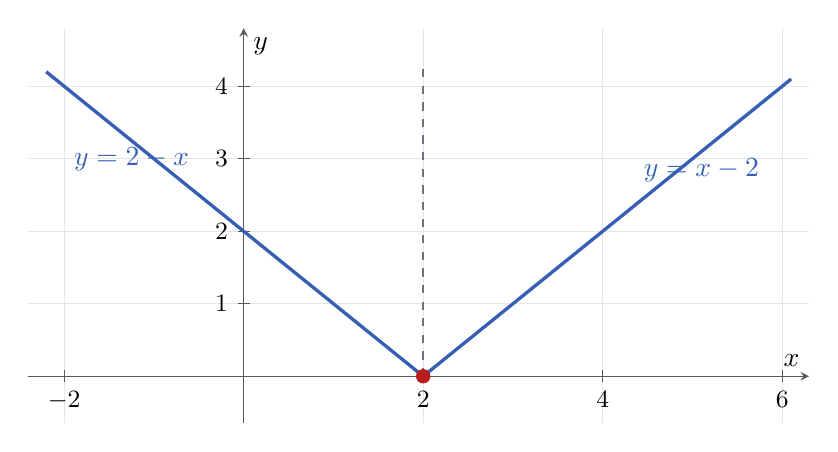
\begin{tikzpicture}
  \begin{axis}[
    width=11.5cm,
    height=6.6cm,
    axis lines=middle,
    xmin=-2.4,
    xmax=6.3,
    ymin=-0.65,
    ymax=4.8,
    xlabel={$x$},
    ylabel={$y$},
    xtick={-2,0,2,4,6},
    ytick={1,2,3,4},
    grid=major,
    grid style={black!10},
    axis line style={black!65},
    tick style={black!65},
    tick label style={font=\small},
    clip=false,
  ]
    \addplot[corba, very thick, domain=-2.2:2, samples=80] {2-x};
    \addplot[corba, very thick, domain=2:6.1, samples=80] {x-2};
    \addplot[only marks, mark=*, mark size=2.4pt, punt]
      coordinates {(2,0)};
    \draw[guia, dashed, thick]
      (axis cs:2,0) -- (axis cs:2,4.25);
    \node[anchor=south east, text=corba] at (axis cs:-0.5,2.7)
      {$y=2-x$};
    \node[anchor=south west, text=corba] at (axis cs:4.35,2.55)
      {$y=x-2$};
  \end{axis}
\end{tikzpicture}
\end{document}
